\documentclass[12pt]{article}
\usepackage[utf8]{inputenc}
\usepackage[english]{babel}
\usepackage[dotinlabels]{titletoc}
\usepackage[nottoc]{tocbibind}
\usepackage{mathptmx}
\usepackage{amsmath, amssymb}
\usepackage{geometry, titlesec, setspace, enumitem}
\usepackage{xcolor, graphicx, caption, subcaption}
\usepackage{hyperref, natbib}
% Journals
\newcommand{\aap}{A\&A}
\newcommand{\aj}{AJ}
\newcommand{\apj}{ApJ}
\newcommand{\araa}{ARA\&A}
\newcommand{\mnras}{MNRAS}
\newcommand{\nat}{Nature}
\newcommand{\pasa}{PASA}
\newcommand{\pasp}{PASP}
\newcommand{\physrep}{PhR}
\newcommand{\prd}{PhRvD}
\newcommand{\rpph}{RPPh}

% Page formatting
\geometry{
	left=1.25in,
	right=1.25in,
	top=1in,
	bottom=1in}
\hypersetup{
	colorlinks=true,
	citecolor=blue,
	filecolor=blue,
	linkcolor=blue,
	urlcolor=blue
}
\setlength{\footnotesep}{10pt}
\setlist{noitemsep}

% Fixing titlesec and hyperref interaction
\makeatletter
\def\ttl@useclass#1#2{%
\@ifstar
{\ttl@labeltrue\@dblarg{#1{#2}}}
{\ttl@labeltrue\@dblarg{#1{#2}}}}
\makeatother

% Image setup
\graphicspath{{figs/}}
\captionsetup[figure]{labelfont={bf}, font={small, stretch=1.3}, name={Figure}, labelsep=period}

% Section and subsection headings
\titleformat{\section}{\normalsize\bfseries\centering}{}{0em}{}
\titleformat{\subsection}{\normalsize\itshape\centering}{}{0.75em}{}
\newcommand{\nocontentsline}[3]{}
\newcommand{\tocless}[2]{\bgroup\let\addcontentsline=\nocontentsline#1{#2}\egroup}
\renewcommand{\contentsname}{Table of Contents}
\renewcommand{\abstractname}{{\normalsize\bfseries\centering{Abstract}}}
\renewcommand{\bibsection}{}

% For figures
\makeatletter
\setlength{\@fptop}{0pt plus 1fil}
\setlength{\@fpbot}{0pt plus 1fil}
\makeatother

% For formatting text and math
\let\vec\mathbf
\newcommand{\code}[1]{{\fontfamily{qcr}\selectfont#1}}
\newcommand{\red}[1]{\textcolor{red}{#1}}
\newcommand{\note}[1]{\textcolor{violet}{#1}}

% Special commands
\newcommand{\HI}{H\,\textsc{i}}
\newcommand{\OI}{O\,\textsc{i}}
\newcommand{\heraqm}{\code{hera\textunderscore qm}}
\newcommand{\herapspec}{\code{hera\textunderscore pspec}}
\newcommand{\herasim}{\code{hera\textunderscore sim}}
\newcommand{\pyuvdata}{\code{pyuvdata}}

\usepackage{lipsum}

\begin{document}
\doublespacing
\begin{center}
Environmental Systematics and the Impact on \\ 21-cm Epoch of Reionization Measurements \\
by \\
Lily Whitler \\
has been approved \\
Spring 2019 \\[0.1\textheight]

\begingroup
\renewcommand{\arraystretch}{0.7}
\begin{tabular}{p{1cm}p{3.5in}p{1cm}}
	& \centering APPROVED: & \\
	& & \\ & & \\
	& \hrulefill & \\
	& \hfill Daniel Jacobs, Director & \\
	& & \\ & & \\
	& \hrulefill & \\
	& \hfill Judd Bowman & \\
	& & \\ & & \\
	& \hrulefill & \\
	& \hfill Adam Beardsley &
\end{tabular} \\[0.075\textheight]
\begin{tabular}{p{1cm}p{3.5in}p{1cm}}
	& \centering ACCEPTED: & \\
	& & \\ & & \\
	& \hrulefill & \\
	& \hfill Dean, Barrett, The Honors College &
\end{tabular}
\endgroup
\end{center}
\thispagestyle{empty}
\newpage
\pagenumbering{arabic}

\begin{center}
	{\Large Environmental Systematics and the Impact on \\ 21-cm Epoch of Reionization Measurements} \\
	by \\
	Lily Whitler \\[0.15\textheight]
	
	A Thesis Presented in Partial Fulfillment \\
	of the Requirements for Graduation from \\
	Barrett, the Honors College \\[0.15\textheight]
	
	Committee: \\
	Daniel Jacobs, Director \\
	Judd Bowman \\
	Adam Beardsley \\[0.2\textheight]
	
	ARIZONA STATE UNIVERSITY \\
	April 2019
\end{center}
\thispagestyle{empty}

\clearpage
\pagenumbering{roman}

\begingroup
\hypersetup{
	citecolor=DarkBlue,
	filecolor=black,
	linkcolor=black,
	urlcolor=DarkBlue
}
\tableofcontents
\listoffigures
\listoftables
\endgroup
\newpage

\begin{abstract}
\end{abstract}

\clearpage
\pagenumbering{arabic}

\section{Introduction} \label{sec:intro}

\subsection{A Brief History of the Universe} \label{subsec:universe}

Immediately after the Big Bang, the universe was a hot plasma of fundamental particles. Now, nearly 14 billion years later, it is populated with a rich variety of \red{objects}, from massive galaxy clusters all the way down to our own solar system and its planets. However, the \red{evolutionary} path the universe took from the Big Bang to now is not entirely clear.

In the early universe, matter was hot and ionized. Photons scattered off of free particles, rendering the universe opaque to electromagnetic radiation. This lasted until approximately 380,000 years after the Big Bang, when the universe had expanded and cooled sufficiently for electrons to become bound to atomic nuclei during recombination. When recombination was complete, photons were able to propagate freely through space, subject only to cosmological redshift. Today, we see photons from this era as the cosmic microwave background (CMB).

Immediately following the release of the CMB and lasting until several hundred million years after the Big Bang was the cosmic Dark Ages. During this era, though photons were free to propagate, no stars, galaxies, or other sources of radiation had yet formed. The only sources of information we have from the Dark Ages are CMB photons and emission from neutral hydrogen.

The transition between the Dark Ages and the subsequent Epoch of Reionization (EoR) was marked by the \red{emergence} of the first luminous sources. During the EoR, ultraviolet (UV) radiation from these objects ionized the intergalactic medium (IGM) around them. The EoR ended when the IGM was fully ionized, thus completing the final major phase change of hydrogen in the universe.

Figure \ref{fig:timeline} shows an illustration of this evolution. The \textit{Planck} satellite and its predecessors, the Cosmic Background Explorer \note{[LW: italicize?]} and \textit{Wilkinson Microwave Anisotropy Probe}, have measured the temperature anisotropies in the CMB, providing a wealth of information about the universe just a few hundred thousand years after its \red{birth}. On the other end of cosmic history, the Hubble Deep Fields have probed some of the oldest known galaxies. However, most of the Dark Ages and EoR still lack observational constraints.

\begin{figure}[tb]
	\centering
	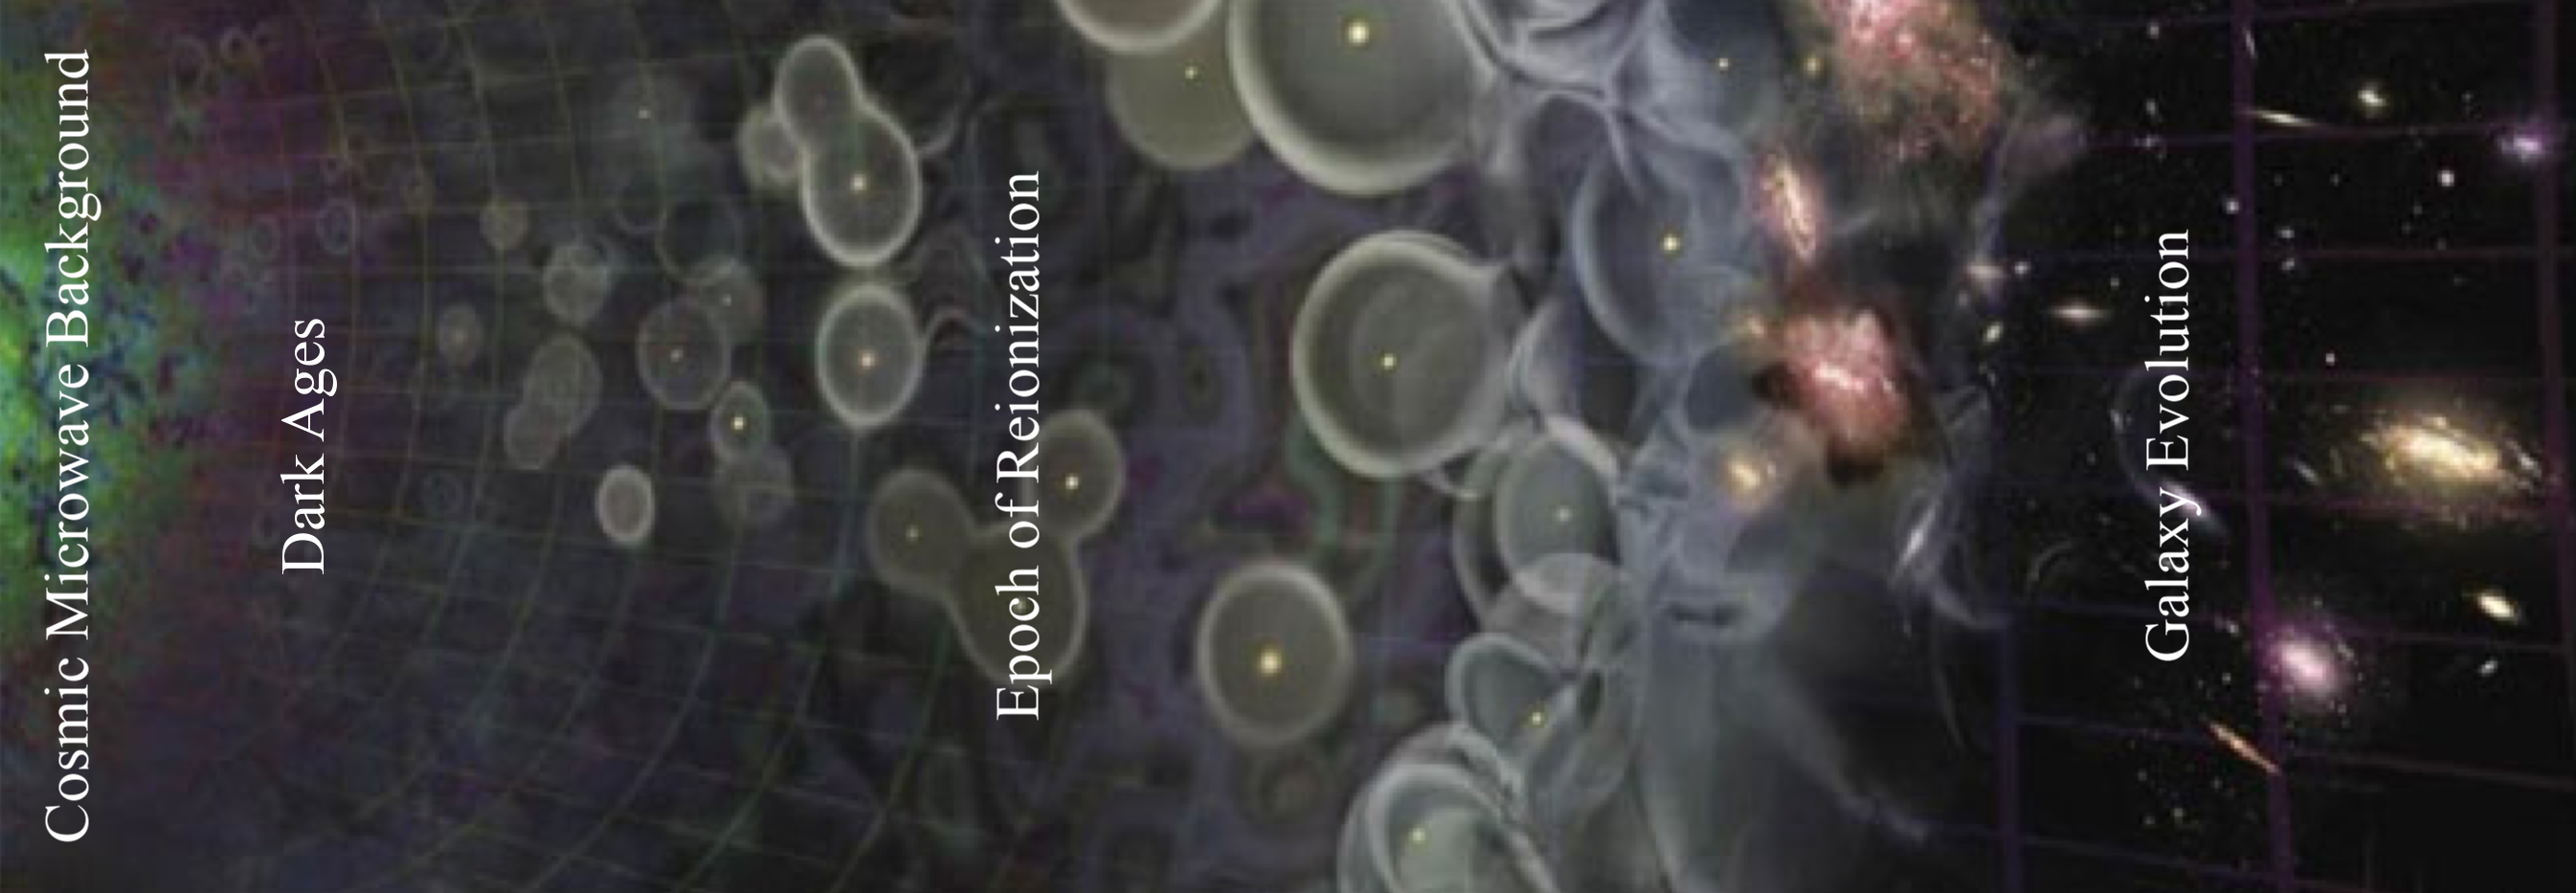
\includegraphics[width=\textwidth]{timeline.png}
	\caption[History of the universe]{A visualization of cosmic evolution. Image modified from \cite{loeb2006}.}
	\label{fig:timeline}
\end{figure}

\subsection{The Epoch of Reionization} \label{subsec:eor}

The EoR is the period in cosmic history during which the intergalactic medium, which had been neutral since recombination, was ionized by the very first luminous sources. This era, along with the Dark Ages, is the bridge between \red{our knowledge of} the CMB and the universe today.

Though the EoR is largely observationally \red{unconstrained}, theoretical studies have constructed a broad \red{account} of the ionization process. UV photons from the earliest stars, galaxies, or quasars ionized the gas in their immediate neighborhood, and as individual objects continue ionizing their surroundings, these bubbles of ionized gas grew in size and eventually began to overlap. As the EoR progressed, the bubbles continued to grow and overlap until the IGM was fully ionized.

This \red{qualitative} picture is generally accepted, but answering more detailed questions such as ``What is the timeline of reionization?'', ``What was the topology? Were there a lot of small bubbles or did a few large ones dominate?'', or even ``What exactly were the ionizing sources?'' will require observations of this era \note{[LW: this sentence can definitely be worded better]}.

\subsection{Observational Constraints on the Epoch of Reionization} \label{subsec:probes}

\cite{fan2006} constrained the end of reionization to be around $z \sim 6$, primarily via observations of high-redshift quasars. In the future, this approach will continue to place tighter \red{limits} on the \red{tail end} of reionization, especially since deep surveys with the upcoming \textit{James Webb Space Telescope} and other ground- and space-based instruments will enable detections of statistically significant samples of these high-redshift objects. However, the quasar luminosity function limits the detection of quasars above $z \gtrsim 7$, thus limiting our ability to probe the earlier part of the EoR with these objects \citep{richards2006, hopkins2007}.

Other probes of the EoR include gamma ray bursts and metal absorption line systems. High-redshift gamma ray bursts exhibit troughs \red{blueward} of Lyman alpha (Ly$\alpha$) in their spectra due to absorption by intervening neutral hydrogen, thus serving as a probe of the ionization state of the IGM \citep[e.g.,][]{gallerani2008}. Early star formation enriches the interstellar medium and the IGM with heavy elements, which can be used either to probe the properties of the stellar populations that ionized the universe or to directly trace the ionization history. For example, \cite{oh2002} \red{proposed} the use of the \OI~line at 1302 \AA, since \OI~and H have almost identical ionization potentials and \OI~is expected to be in tight charge exchange equilibrium with H.

Both the large-scale polarization of the CMB and the small-scale kinetic Sunyaev-Zel'dovich (kSZ) effect place some constraints on the onset and topography of reionization \citep{fan2006}. CMB photons undergo Thomson scattering off of free electrons produced by the ionization of hydrogen which causes the emission to polarize. This interaction can be quantified by the optical depth of reionization, and thus the redshift. Primary CMB anisotropies are suppressed by this polarization, so measuring the polarization caused by CMB photons Thomson scattering during reionization constrains the onset of the EoR \citep[e.g.,][]{zaldarriaga1997, roy2018}. The kSZ effect, on the other hand, is due to inverse Compton scattering of ionized electrons in the IGM and introduces secondary temperature anisotropies on small angular scales, which is a tracer of the \red{patchiness} of reionization \citep{fan2006, park2013, roy2018}.

As useful as the CMB is as a probe of the EoR, it is essentially a two-dimensional snapshot of the universe taken at one time in cosmic history. Although the CMB has imprints of other eras, specifically the EoR, on it, a three-dimensional map would contain much information. \note{[LW: Transitions are good. I should have some. But moving onto 21-cm stuff for now...]}

\subsection{21-cm Cosmology} \label{subsec:21cm}

Neutral hydrogen emits a photon with a wavelength of 21 centimeters during its ``spin-flip transition.'' In the ground state of neutral hydrogen, an electron is bound to a proton, each of which has an intrinsic quantum spin due to their magnetic dipole moments. The spin of the electron can be either parallel or antiparallel to the proton's spin, and the parallel state is slightly higher in energy. The transition from the parallel to the antiparallel state is called the spin-flip transition and results in the emission of a 21-cm photon. A \red{cartoon} of this process is in Figure \ref{fig:spin_flip}.

The energy difference between these two states is $\sim 5.87$ $\mu$eV, a tiny fraction of the 13.6 eV necessary to ionize hydrogen once, making the 21-cm line one of the only ways to probe the very low-energy environment of the Dark Ages and early stages of the EoR. Due to the expansion of the universe, the observed wavelength of the 21-cm line is redshifted to longer wavelengths, which can be traced back to a specific time in cosmic history. This redshift evolution provides a full three-dimensional probe of the EoR. Theoretical studies of the EoR place the EoR approximately between $z \sim 6 - 20$ \note{[LW: 15? 20? Unsure of the exact theoretical view on the timeline. Also, citations.]}, which corresponds to observed wavelengths of approximately 1.5 -- 4.5 meters. The spin flip transition has a very small transition rate of $2.9 \times 10^{-15}$ s$^{-1}$, or about one transition every 10 million years, but fortunately, hydrogen is incredibly ubiquitous in the universe so we can still use this line as an EoR probe.

\note{[LW: 21-cm tomography and fluctuations on spatial scales?]}

Actually measuring 21-cm emission from the EoR, however, is an exercise in extreme precision. Synchrotron emission from our own galaxy and other extragalactic sources dominates the frequency band of interest, creating foregrounds that are several orders of magnitude brighter than the 21-cm signal is expected to be. These foregrounds are the primary challenge that all 21-cm experiments must overcome to detect the EoR. However, the environment and the instrument can introduce other \red{systematics}, such as radio frequency interference (RFI), ionospheric effects, and signal reflections, that further complicate the measurement.

\begin{figure}[t]
	\centering
	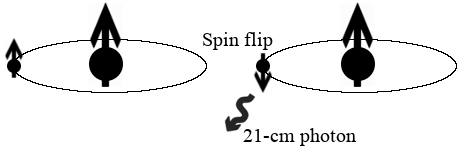
\includegraphics[width=0.55\textwidth]{spin_flip.png}
	\caption[The spin-flip transition of neutral hydrogen]{A \red{cartoon} of the spin-flip transition of neutral hydrogen. Initially, the spin of the electron is parallel with that of the proton---both are in a ``spin up'' state. This initial state is at a higher energy than when the spin of the electron and proton are antiparallel. The transition occurs when the spin of the electron flips from up to down, emitting a photon with a wavelength of 21 cm.}
	\label{fig:spin_flip}
\end{figure}

\subsection{Radio Frequency Interference} \label{subsec:rfi}

Interference from sources including FM radio, satellite and aircraft communications, television transmissions, and even nearby weather events (e.g., lightning) is exceptionally bright and can easily contaminate the results of any cosmological measurement. \red{Unfortunately}, since it is typically man-made, it is also everywhere that humans are.

There are a few ways to mitigate RFI. First, instruments can be built in remote areas to minimize contact with human-made interference. Then, RFI can be removed after taking observations with software that detects and masks out (``flags'') data it identifies as being contaminated. Steps further along in the data reduction and analysis process ignore this flagged data.

There are currently several radio interferometers making observations towards a 21-cm power spectral EoR detection, some of which are located in remote places of the world and all \red{(I think)} of which use some sort of RFI excision software. \note{[LW: Remember what I said earlier about transitions?]}

\subsection{The Hydrogen Epoch of Reionization Array} \label{subsec:hera}

\begin{figure}[tb]
	\centering
	\begin{subfigure}{0.48\textwidth}
		\centering
		{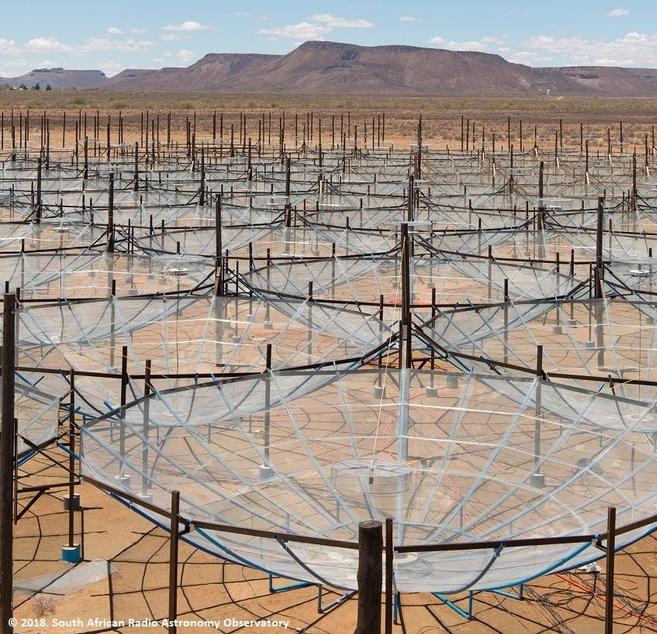
\includegraphics[width=\textwidth]{hera.png}}
	\end{subfigure} \hfill
	\begin{subfigure}{0.48\textwidth}
		\centering
		{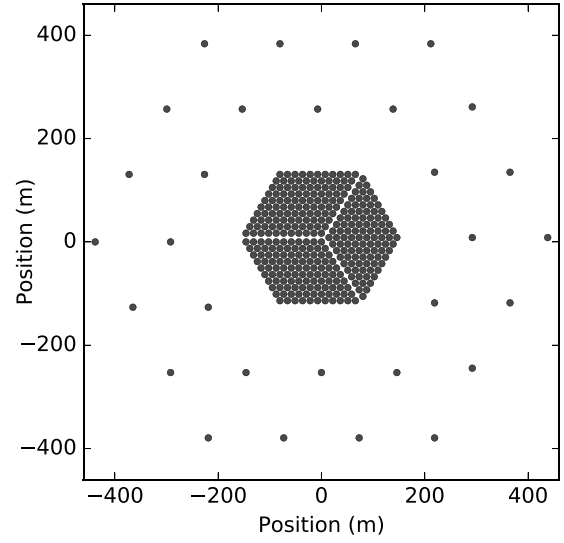
\includegraphics[width=\textwidth]{hera_map.png}}
	\end{subfigure}
	\caption[The Hydrogen Epoch of Reionization Array]{Left: A photo of HERA as of late 2017 -- early 2018. HERA will observe the periods prior to and during the EoR via the redshifted 21-cm line from the IGM. Image courtesy of the South African Radio Astronomy Observatory. Right: A map of the completed array, composed of 320 central elements and 30 outriggers \citep{deboer2017}.}
	\label{fig:hera}
\end{figure}

HERA (left panel of Figure \ref{fig:hera}) is one of several radio interferometers designed to study the large-scale structure during the EoR via measurements of the redshifted 21-cm line \citep{deboer2017}---others include the Low Frequency Array \citep[LOFAR;][]{vanHaarlem2013} and the Murchison Widefield Array \citep[MWA;][]{tingay2013}. HERA builds upon preceding instruments, such as the MWA and the Donald C. Backer Precision Array for Probing the Epoch of Reionization \citep[PAPER;][]{parsons2010}, and will pave the way for future experiments such as the Square Kilometer Array \cite[SKA; e.g.,][]{mellema2013}.

When complete, HERA will be \red{composed} of 350 14-meter dishes with a dense 320-element hexagonal core and 30 outriggers (right panel of Figure \ref{fig:hera}). The dense \red{configuration} was chosen to maximize sensitivity to the diffuseness of the 21-cm signal, which will be sampled primarily by short baselines. The redundancy of the hexagonal shape increases sensitivity and the efficacy of the delay spectrum approach for separating and \textit{avoiding} foreground-contaminated modes \note{[LW: A PAPER thing---citation?]} and allows for the redundant calibration technique developed and pioneered in \cite{liu2010} and \cite{zheng2014}. \note{[LW: I need to expand on a lot of this (like the delay spectrum...)]}

HERA's first scientific observing campaign took place from September 2017 to the beginning of April 2018, with the first calibrated, LST-binned internal data release, H1C (HERA with $\sim 100$ antennas) IDR 2.1, occurring in June 2018 (public HERA memo \href{http://reionization.org/wp-content/uploads/2018/07/IDR2.1_Memo_v2.html}{\#45}). A broad overview of the data processing can be found in section 5 in the same memo; key \red{points} include several calibration steps (e.g., redundant calibration and absolute gain calibration) and flagging RFI.

\section{Methods} \label{sec:methods}

\subsection{RFI Excision Strategies} \label{subsec:rfi_excision}

\begin{figure}[p]
	\centering
	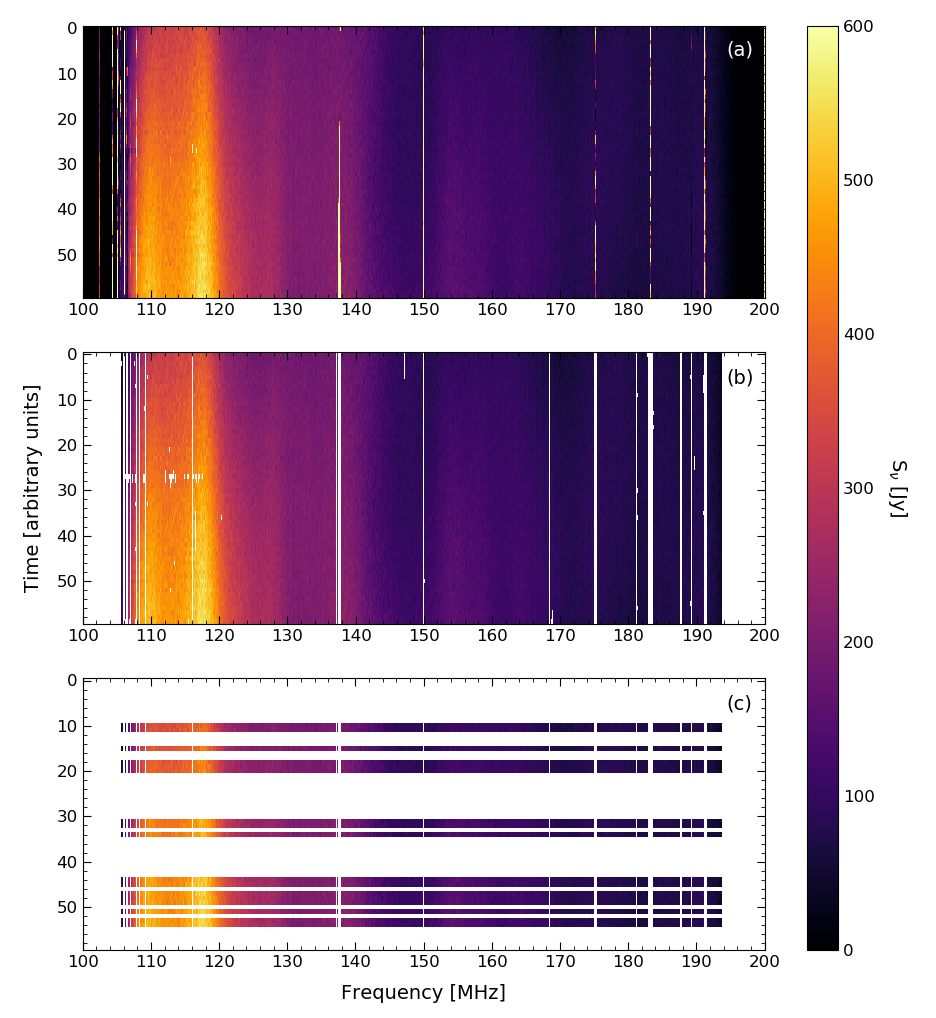
\includegraphics[width=\textwidth]{flagging_steps.png}
	\caption[Steps for flagging RFI]{An example of the process of flagging RFI from (a) unflagged visibilities to (b) XRFI flags, and finally (c) broadcasted flags. The red arrows in (b) indicate frequency pixels with enough flags to flag the entire channel as determined by the procedure described in Section \ref{subsec:rfi_excision}, with the flagged channels shown by the red lines in (c). Similarly, grey arrows and lines indicate the initial flags and subsequent broadcasting for time integrations that were completely flagged.}
	\label{fig:rfi_flagging}
\end{figure}

The H1C IDR 2.1 data reduction pipeline utilizes code developed for HERA quality \red{assurance} (\heraqm\footnote{\url{https://github.com/HERA-team/hera_qm}}) to identify and flag RFI. The entire flagging pipeline, XRFI, functions as follows:

\begin{enumerate}
	\item Data for individual antennas or baseline are detrended with a median filter by calculating the difference between the data and median and dividing by the noise.
	\item The same data are flagged based on user-defined thresholds.
	\item Flags from individual antennas/baselines are averaged over time, thresholded, and flagged again over a full file.
	\item The data are delay filtered to remove foregrounds. \note{[LW: This is awful and needs explanation.]}
	\item Visibilities are flagged following the procedure in steps 1 -- 3 and combined into final observation flags.
\end{enumerate}

After flagging with XRFI, the flags are broadcast such that the patterns are time independent for a given baseline and spectral window. For a given frequency pixel, also called a channel, in the selected spectral window, if the total fraction of flagged times in that channel exceeds a predefined threshold, then the entire channel is flagged. Otherwise, if the flagged times in the channel do not exceed the threshold, any time integrations that contain flags are flagged for all frequencies in the spectral window. This process is carried out for each frequency pixel until all flags are time independent. \note{[LW: Might want to go into why this is necessary.]} Figure \ref{fig:rfi_flagging} shows an example of this flagging algorithm in \red{practice}, progressing from visibilities to XRFI flags to broadcasted flags.

\note{[LW: Talk about what I actually did with flagging...]}

\subsection{The Power Spectrum} \label{subsec:calc_ps}

Conventionally, the 21-cm power spectrum $P_{21}\left(\vec{k}\right)$ is mathematically defined as
\begin{equation}
\left\langle \widetilde{T}_b\left(\vec{k}\right) \widetilde{T}_b^*\left(\vec{k'}\right) \right\rangle = \left(2\pi\right)^3 \delta\left(\vec{k} - \vec{k'}\right) P_{21}\left(\vec{k}\right)
\label{eqn:P21}
\end{equation}
where $\widetilde{T}_b\left(\vec{k}\right)$ is the 3D spatial Fourier transform of the brightness temperature distribution on the sky and $\delta$ is the Dirac delta function. However, Equation \ref{eqn:P21} \red{includes} two continuous functions, $T_b$ and $P_{21}$, which must be discretized to be computational feasible.

The HERA collaboration's power spectrum estimation code, \herapspec\footnote{\url{https://github.com/HERA-team/hera_pspec}}, uses the same optimal quadratic estimator as was used for PAPER analysis \citep{ali2015}, with further \red{information} in, e.g., \cite{tegmark1997}, \cite{tegmark1998}, \cite{liu2011}. Thus equipped with a feasible way of estimating the 21-cm power spectrum, I use data flagged as described in Section \ref{subsec:rfi_excision} to estimate a \red{delay} spectrum.

\note{[LW: I don't know how much I want to write in this section because I don't have the most rigorous understanding of what's going on.]}

\begin{figure}[t]
	\centering
	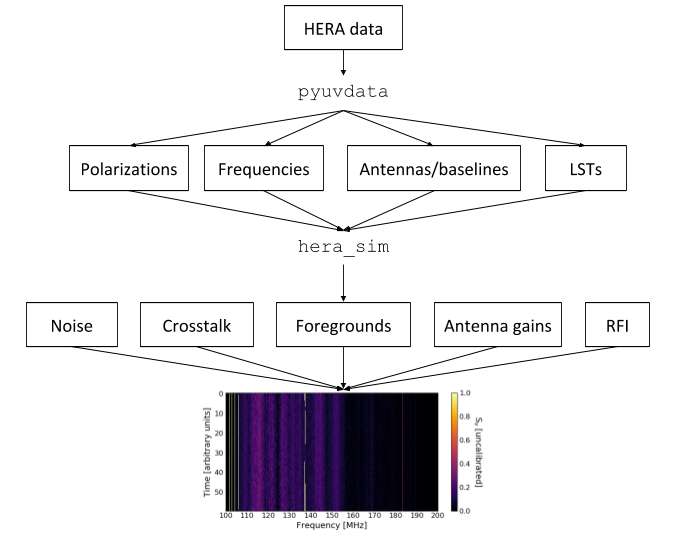
\includegraphics[width=\textwidth]{sim_flow.png}
	\caption[Flowchart of the process of modelling HERA data]{A flowchart of the process used to simulate HERA data. In particular, the foreground model is based off of parameters from real data. RFI, noise, antenna gains, and crosstalk (when the signal from two antennas gets erroneously correlated) calculated independently by \herasim~are added to yield a mock dataset.}
	\label{fig:sim_flow}
\end{figure}

\begin{figure}[p]
	\centering
	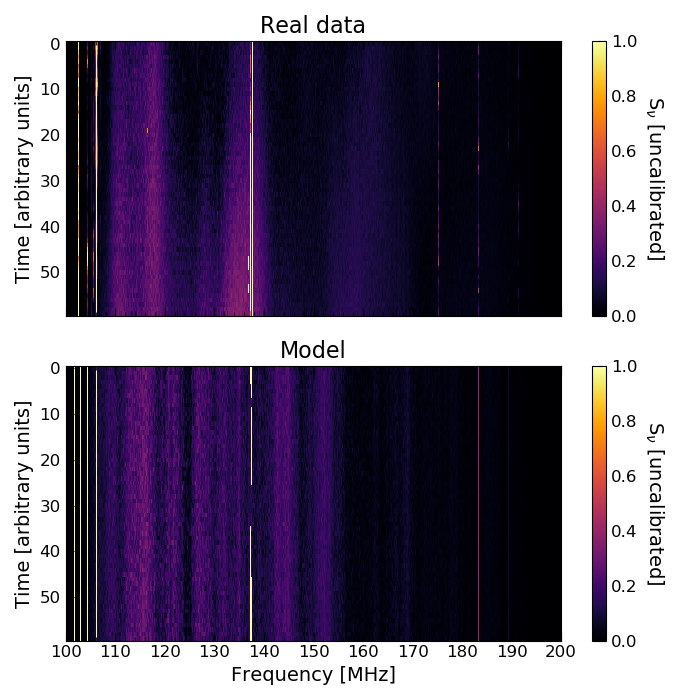
\includegraphics[width=\textwidth]{sim_comparison.png}
	\caption[Comparison of simulated and real data]{A comparison between the model data and the real data used to obtain parameters for the simulation for one 14-meter baseline. Particular interference features to note include the Orbcomm satellite constellation downlink at approximately $137$ MHz, broadcasts from FM radio at lower frequencies, and TV transmissions at higher frequencies.}
	\label{fig:sim_comparison}
\end{figure}

\subsection{Modelling HERA Data} \label{subsec:modelling}

In order to perform tests in a more controlled setting, I modelled HERA data with the simple visibility simulator \herasim\footnote{\url{https://github.com/HERA-team/hera_sim}}. Using the package \pyuvdata\footnote{\url{https://github.com/RadioAstronomySoftwareGroup/pyuvdata}} as an interface between HERA data files and \herasim, I used real observation parameters such as observed frequencies, local sidereal times (LSTs), antenna positions, baselines, and polarizations as input\red{s} to the simulator. This was done in an effort to create realistic \red{realizations} of what HERA might actually observe. Figure \ref{fig:sim_flow} shows a visualization of this process and Figure \ref{fig:sim_comparison} shows an example of the resulting model and the uncalibrated real data scaled to match the model.

Since RFI is the focus of this work, I took special care to \red{at least approximately} match the RFI patterns in the simulation to those present in real data. In particular, I focused on matching three interference features: the Orbcomm satellite constellation downlink at $137 - 138$ MHz, FM radio broadcasts at frequencies less than $108$ MHz, and the occasional VHF TV transmission above $\sim 175$ MHz. All of these can be seen as thin vertical lines in Figure \ref{fig:sim_comparison}.

\section{Results}

\subsection{RFI Excision Tests} \label{subsec:rfi_tests}

\begin{enumerate}
	\item Different time thresholds for broadcasting
	\item Flagging additional adjacent channels
	\item Flagging additional non-adjacent channels
\end{enumerate}

\subsection{Model Results} \label{subsec:model_results}

\begin{enumerate}
	\item Going all the way back to XRFI flagging strategies through broadcasting
\end{enumerate}

\section{Conclusions}

The Epoch of Reionization and the preceding Dark Ages are among the last unexplored periods of our universe's history. Filling in the story of cosmic evolution with the timeline and topography of the EoR will provide the beginnings of a much-needed bridge between the CMB and the rich structure we see today. Measuring and analyzing the power spectrum of the 21-cm with HERA, among other current and next-generation instruments, will be a key component of building that bridge.

Several challenges, not the least of which are bright radio foregrounds, stand between us and studying the EoR with this method. However, though radio foregrounds are the largest obstacle, even a single \red{misunderstood} or uncorrected systematic error makes a detection more difficult. Such systematics can range from instrumental effects that aren't quite calibrated correctly to man-made interference.

Towards the goal of making this detection, I have focused on characterizing the effects of RFI on the power spectrum. In particular, I have used methods and techniques already developed by the HERA collaboration in an attempt to recreate the circumstances under which future analyses will be undertaken. This includes everything from initial RFI identification and flagging to the final estimation of the power spectrum.

Future work:
\begin{enumerate}
	\item Flagging over subband
	\item Analytical representation of flag broadcasting (can we even optimize that?)
\end{enumerate}

\bibliographystyle{aasjournal}
\bibliography{refs}

\begin{figure}[p]
	\centering
	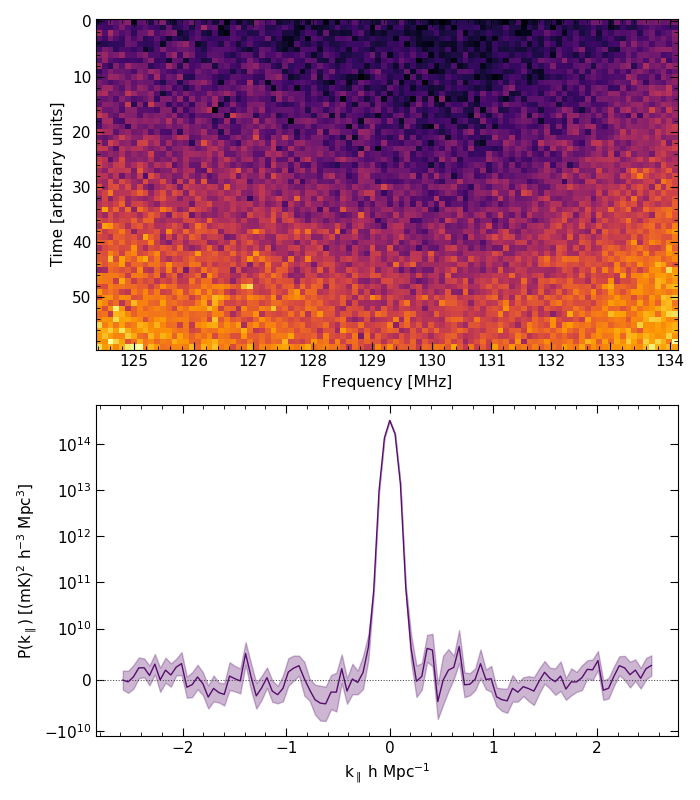
\includegraphics[width=\textwidth]{42378_noflags.png}
	\caption[Original power spectrum]{Caption}
	\label{fig:noflags}
\end{figure}

\begin{figure}[p]
	\centering
	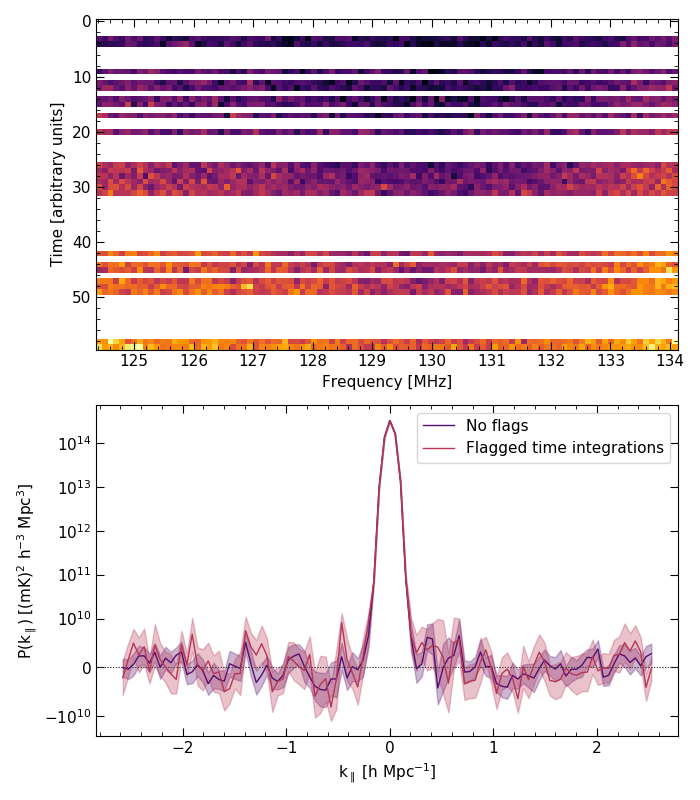
\includegraphics[width=\textwidth]{42378_timeflags.png}
	\caption[Power spectrum calculated with data flagged only in time]{Caption}
	\label{fig:time_flags}
\end{figure}

\begin{figure}[p]
	\centering
	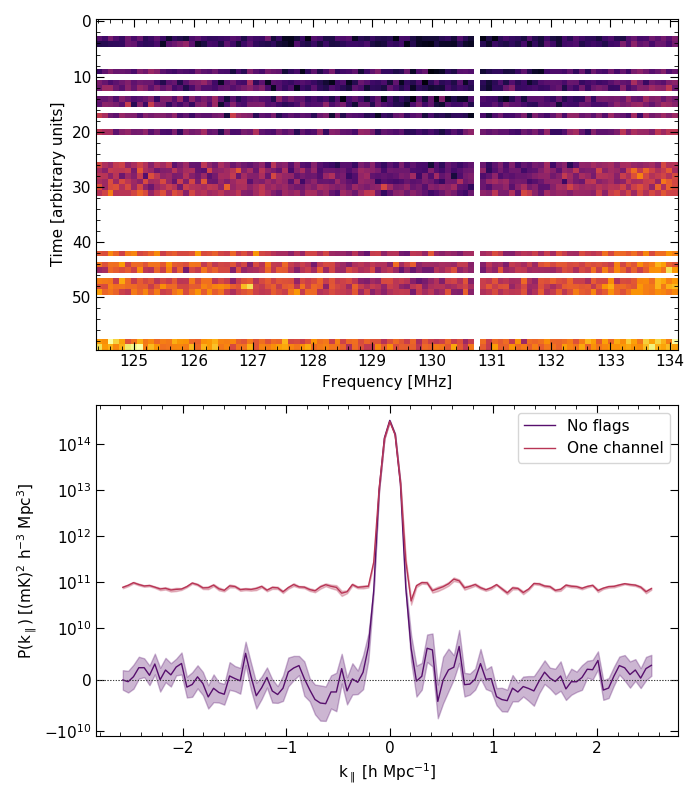
\includegraphics[width=\textwidth]{42378_flag315.png}
	\caption[Power spectrum calculated with flagged time integrations and one flagged channel]{Caption}
	\label{fig:flag_chan315}
\end{figure}

\begin{figure}[p]
	\centering
	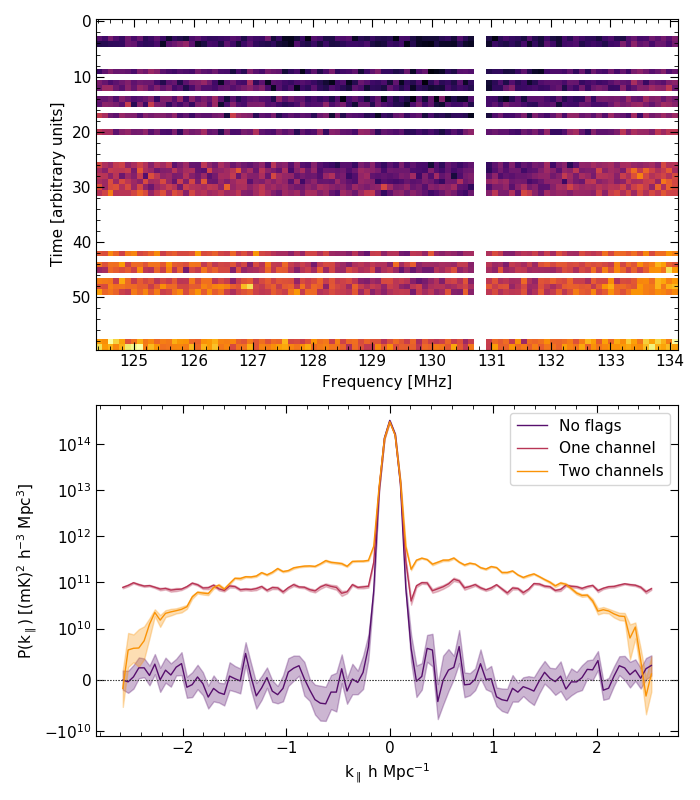
\includegraphics[width=\textwidth]{42378_flag315_316.png}
	\caption[Power spectrum calculated with flagged time integrations and two contiguous flagged channels]{Caption}
	\label{fig:flag_chan315_316}
\end{figure}

\begin{figure}[p]
	\centering
	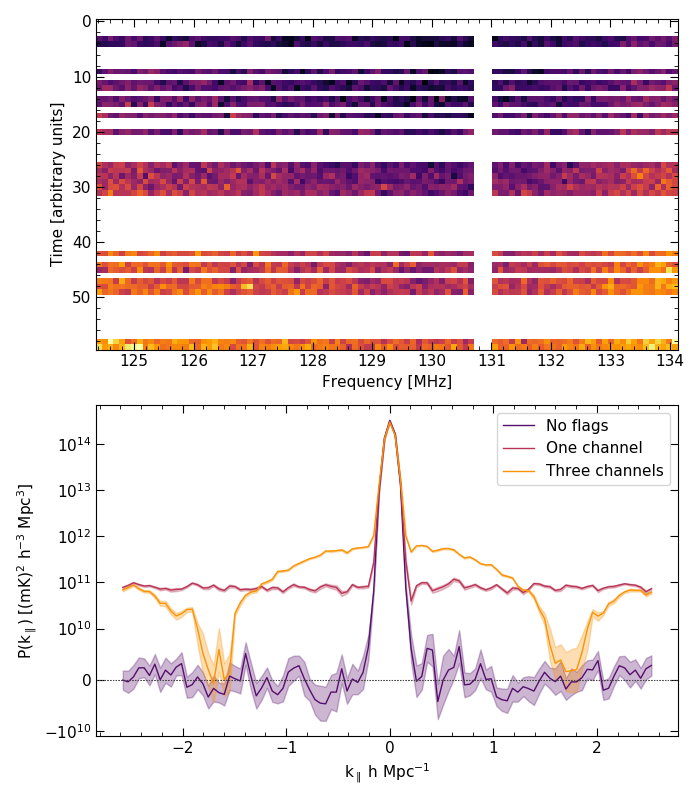
\includegraphics[width=\textwidth]{42378_flag315_317.png}
	\caption[Power spectrum calculated with flagged time integrations and three contiguous flagged channels]{Caption}
	\label{fig:flag_chan315_317}
\end{figure}

\begin{figure}[p]
	\centering
	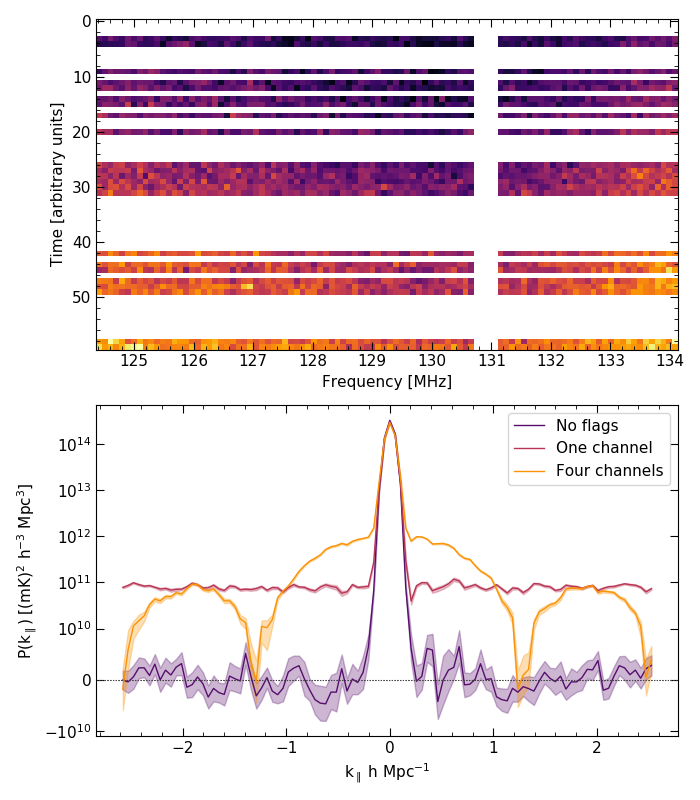
\includegraphics[width=\textwidth]{42378_flag315_318.png}
	\caption[Power spectrum calculated with flagged time integrations and four contiguous flagged channels]{Caption}
	\label{fig:flag_chan315_318}
\end{figure}

\begin{figure}[p]
	\centering
	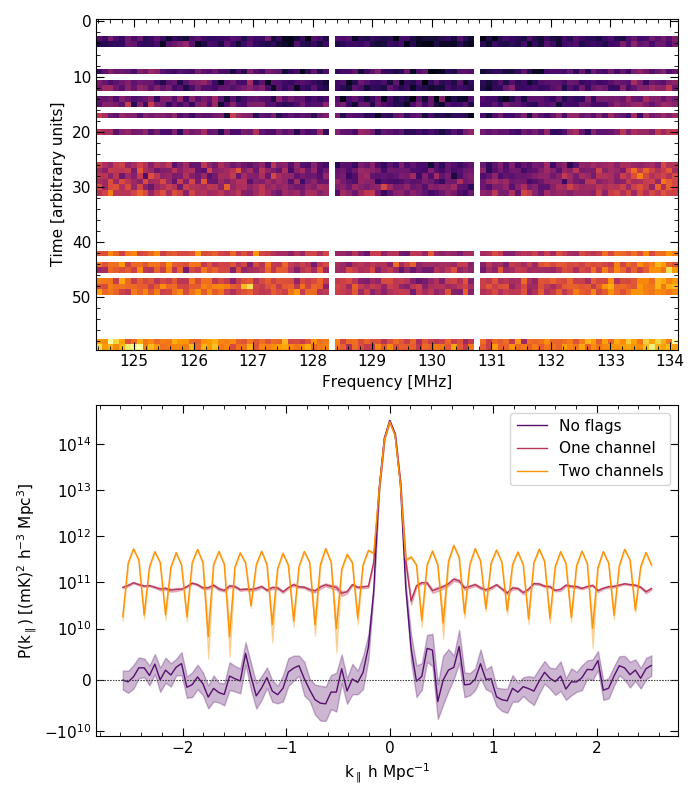
\includegraphics[width=\textwidth]{42378_flag290_315.png}
	\caption[Power spectrum calculated with flagged time integrations and two non-contiguous flagged channels]{Caption}
	\label{fig:flag_chan290_315}
\end{figure}

\begin{figure}[p]
	\centering
	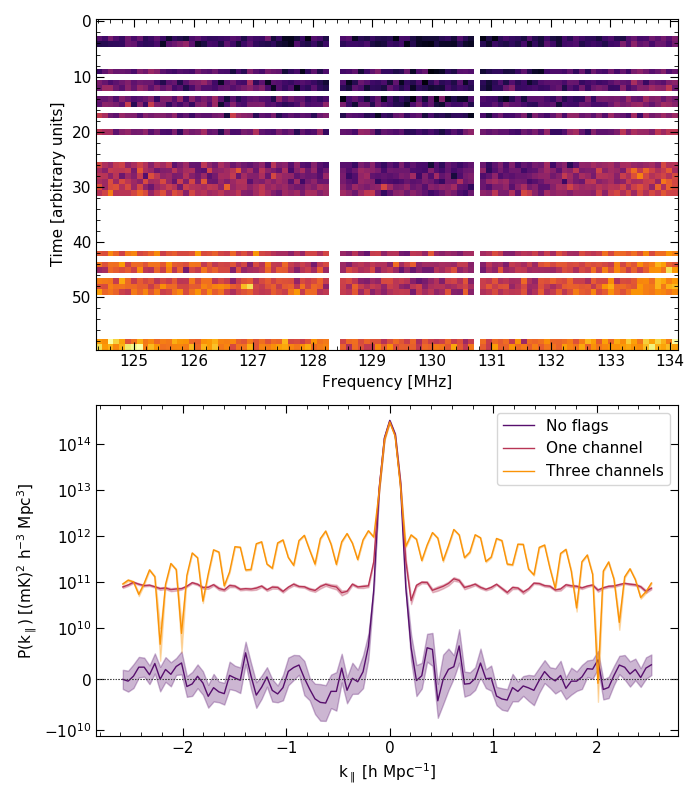
\includegraphics[width=\textwidth]{42378_flag290_291_315.png}
	\caption[Power spectrum calculated with flagged time integrations and three flagged channels (two contiguous, one not)]{Caption}
	\label{fig:flag_chan290_291_315}
\end{figure}

\begin{figure}[p]
	\centering
	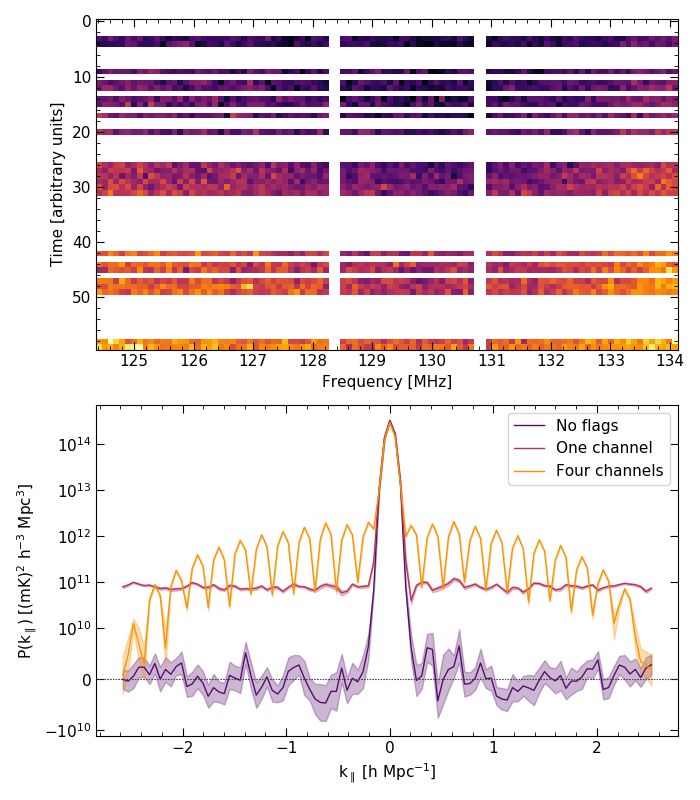
\includegraphics[width=\textwidth]{42378_flag290_291_315_316.png}
	\caption[Power spectrum calculated with flagged time integrations and four flagged channels (two blocks of two channels)]{Caption}
	\label{fig:flag_chan290_291_315_316}
\end{figure}

\begin{figure}[p]
	\centering
	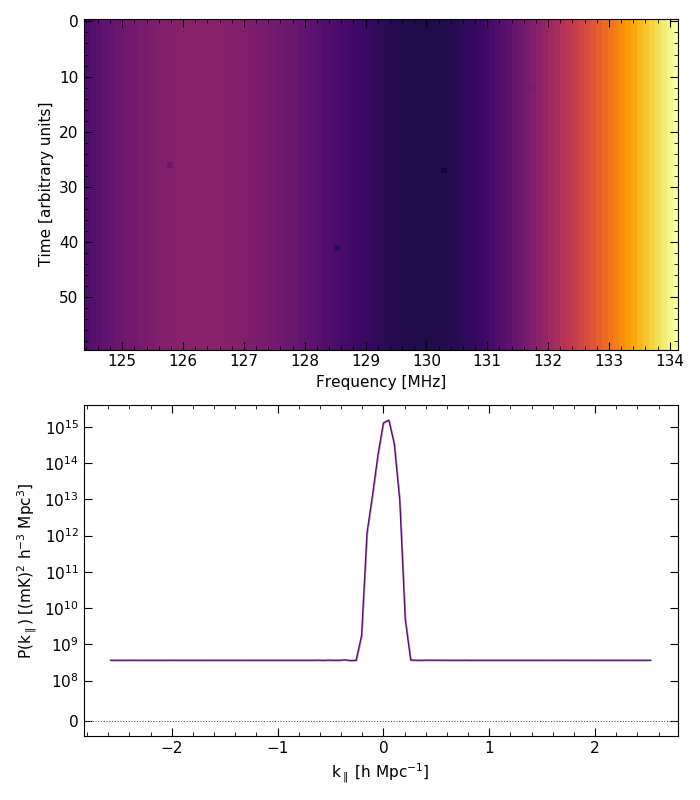
\includegraphics[width=\textwidth]{49088_sim_noflags.png}
	\caption[Original model power spectrum (only foregrounds)]{Caption}
	\label{fig:sim_noflags}
\end{figure}

\begin{figure}[p]
	\centering
	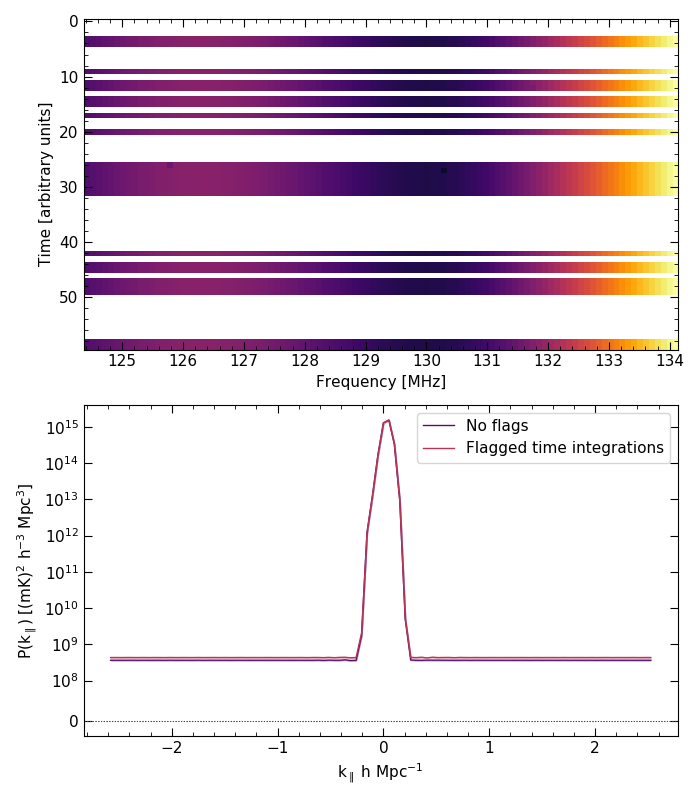
\includegraphics[width=\textwidth]{49088_sim_timeflags.png}
	\caption[Model power spectrum calculated with data flagged only in time]{Caption}
	\label{fig:sim_time_flags}
\end{figure}

\begin{figure}[p]
	\centering
	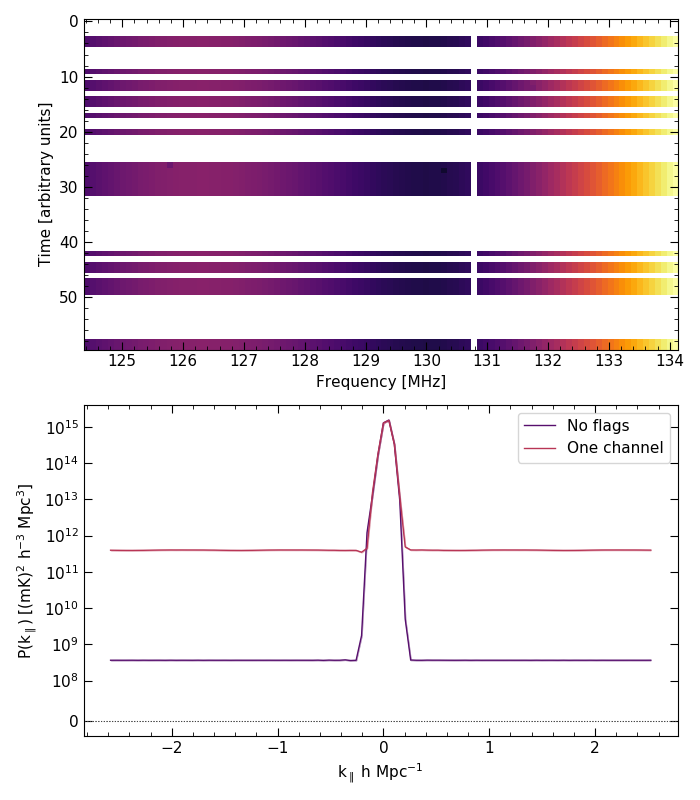
\includegraphics[width=\textwidth]{49088_sim_flag315.png}
	\caption[Model power spectrum calculated with flagged time integrations and one flagged channel]{Caption}
	\label{fig:sim_flag_chan315}
\end{figure}

\begin{figure}[p]
	\centering
	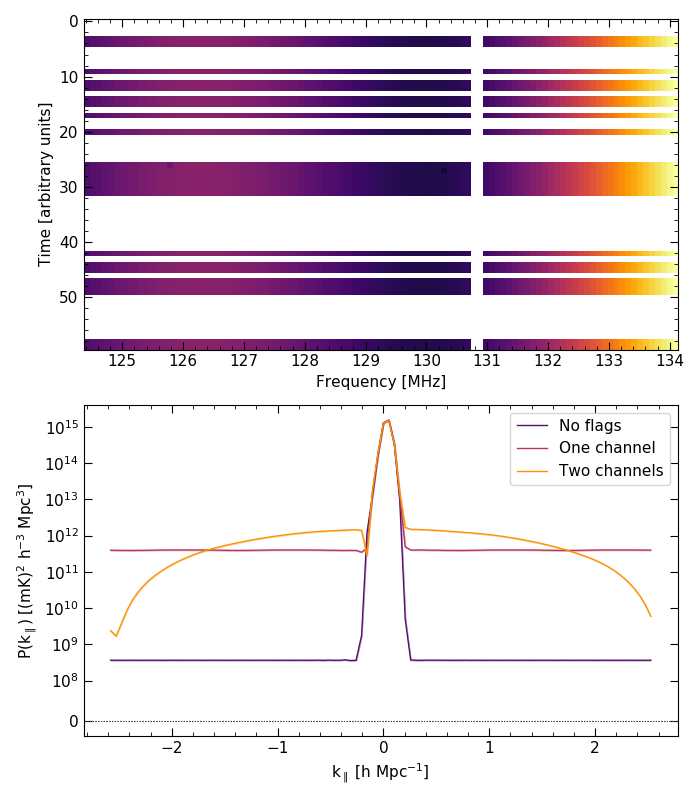
\includegraphics[width=\textwidth]{49088_sim_flag315_316.png}
	\caption[Model power spectrum calculated with flagged time integrations and two contiguous flagged channels]{Caption}
	\label{fig:sim_flag_chan315_316}
\end{figure}

\begin{figure}[p]
	\centering
	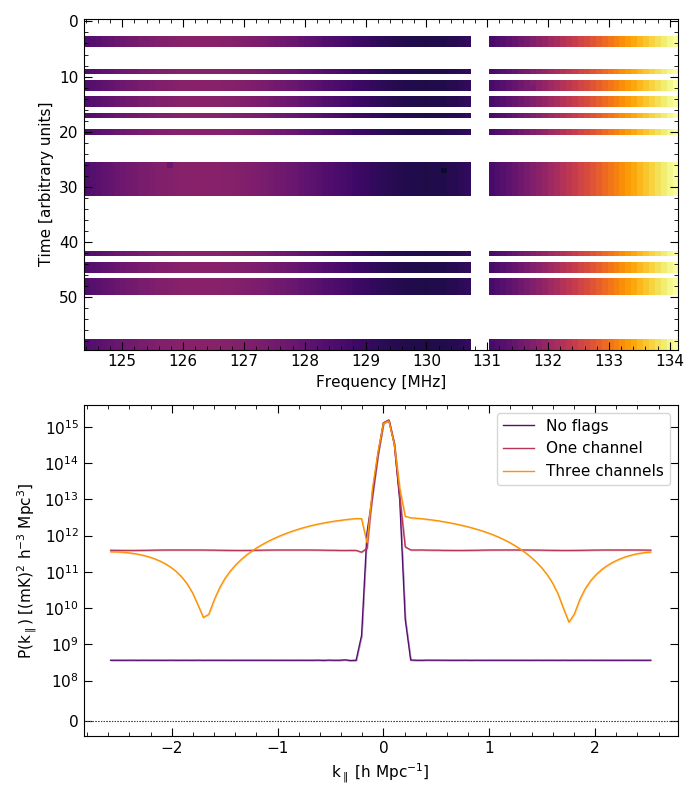
\includegraphics[width=\textwidth]{49088_sim_flag315_317.png}
	\caption[Model power spectrum calculated with flagged time integrations and three contiguous flagged channels]{Caption}
	\label{fig:sim_flag_chan315_317}
\end{figure}

\begin{figure}[p]
	\centering
	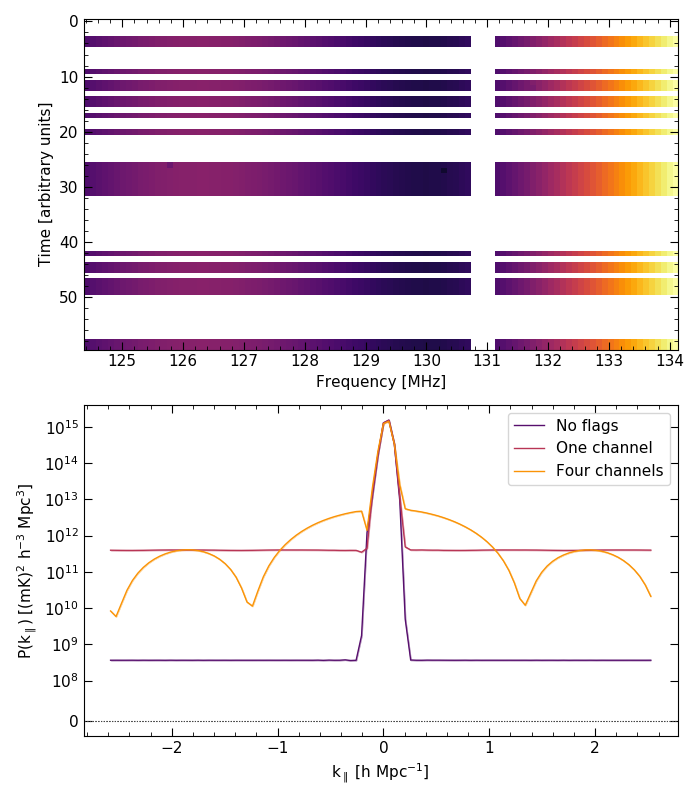
\includegraphics[width=\textwidth]{49088_sim_flag315_318.png}
	\caption[Model power spectrum calculated with flagged time integrations and four contiguous flagged channels]{Caption}
	\label{fig:sim_flag_chan315_318}
\end{figure}

\begin{figure}[p]
	\centering
	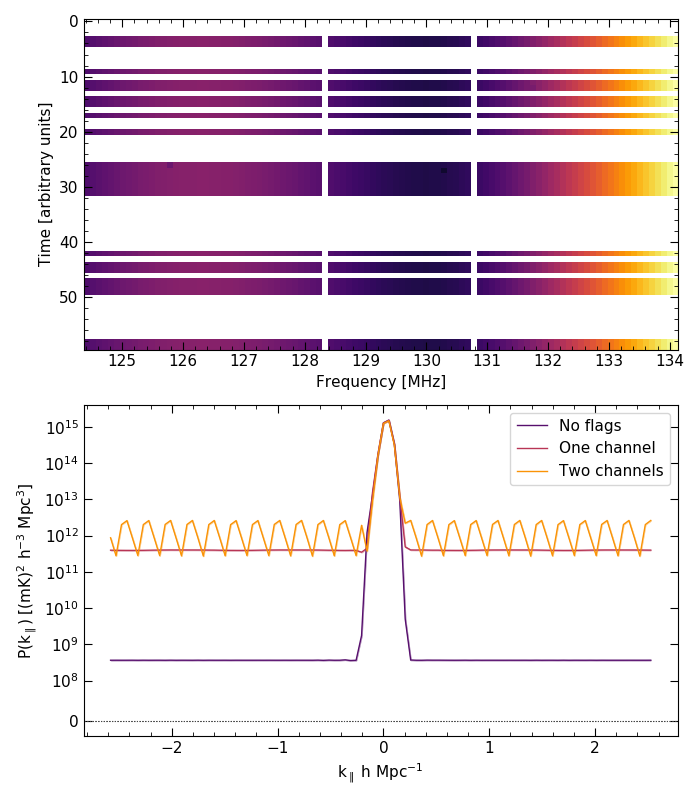
\includegraphics[width=\textwidth]{49088_sim_flag290_315.png}
	\caption[Model power spectrum calculated with flagged time integrations and two non-contiguous flagged channels]{Caption}
	\label{fig:sim_flag_chan290_315}
\end{figure}

\begin{figure}[p]
	\centering
	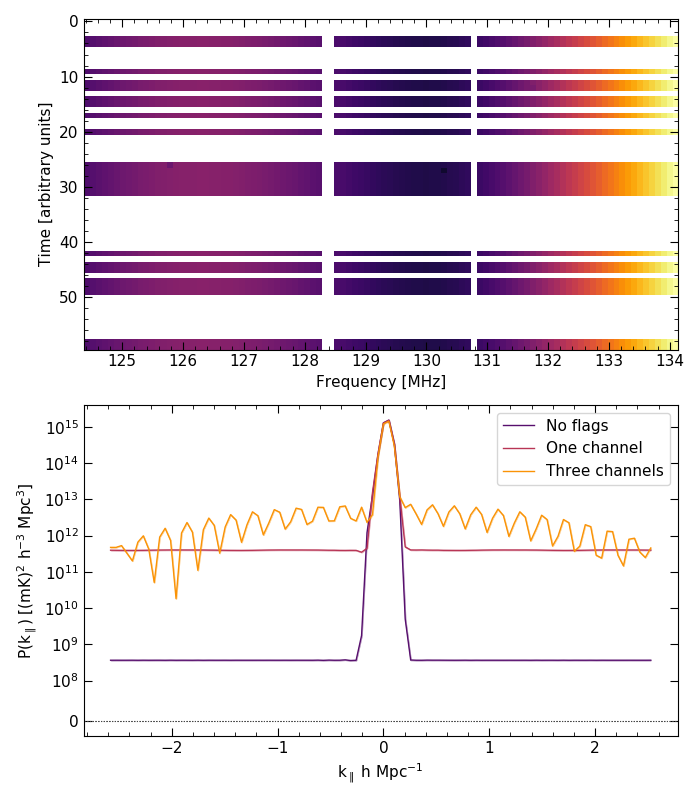
\includegraphics[width=\textwidth]{49088_sim_flag290_291_315.png}
	\caption[Model power spectrum calculated with flagged time integrations and three flagged channels (two contiguous, one not)]{Caption}
	\label{fig:sim_flag_chan290_291_315}
\end{figure}

\begin{figure}[p]
	\centering
	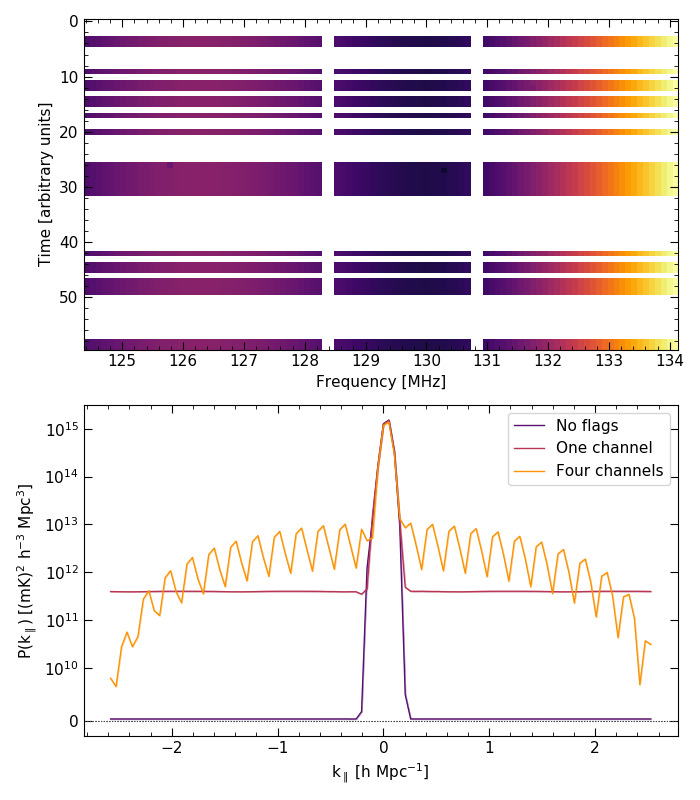
\includegraphics[width=\textwidth]{49088_sim_flag290_291_315_316.png}
	\caption[Model power spectrum calculated with flagged time integrations and four flagged channels (two blocks of two channels)]{Caption}
	\label{fig:sim_flag_chan290_291_315_316}
\end{figure}
\end{document}